\documentclass[a4paper]{jpconf}

\usepackage{graphicx}

\usepackage{hyperref}

\usepackage{cite}

\usepackage{amsmath}

\usepackage{bm}

\newcommand{\maestro}{{\sffamily Maestro}}
\newcommand{\castro}{{\sffamily Castro}}
\newcommand{\starkiller}{{\sffamily StarKiller}}
\newcommand{\starlord}{{\sffamily StarLord}}
\newcommand{\nyx}{{\sffamily Nyx}}
\newcommand{\amrex}{{\sffamily AMReX}}

\newcommand{\Uc}{{\,\bm{\mathcal{U}}}}
\newcommand{\Adv}[1]{{\left [\boldsymbol{\mathcal{A}} \left(#1\right)\right]}}
\newcommand{\Advt}[1]{{\left [\mathcal{\tilde{A}} \left(#1\right)\right]}}
\newcommand{\Advs}[1]{\boldsymbol{\mathcal{A}} \left(#1\right)}



\newcommand{\cpp}{C\nolinebreak\hspace{-.05em}\raisebox{.4ex}{\tiny\bf +}\nolinebreak\hspace{-.10em}\raisebox{.4ex}{\tiny\bf +}}

\usepackage{color}
\setlength{\marginparwidth}{0.75in}
\newcommand{\MarginPar}[1]{\marginpar{\vskip-\baselineskip\raggedright\tiny\sffamily\hrule\smallskip{\color{red}#1}\par\smallskip\hrule}}

\newcommand{\apj}{Astrophysical Journal}
\newcommand{\aap}{Astronomy and Astrophysics}
\newcommand{\mnras}{Monthly Notices of the Royal Astronomical Society}
\newcommand{\prd}{Physical Review D}
\newcommand{\apjs}{Astrophysical Journal Supplement}

\begin{document}

\title{Toward Resolved Simulations of Burning Fronts in Thermonuclear
       X-ray Bursts}

\author{M. Zingale$^1$,
        K.~Eiden$^1$,
        Y.~Cavecchi$^2$,
        A.~Harpole$^1$,
        J.~B. Bell$^2$,
        M.~Chang$^1$,
        M.~P. Katz$^5$,
        C.~M. Malone$^6$, 
        A.~J. Nonaka$^2$,
        D.~E. Willcox$^2$, and
        W. Zhang$^2$}

\address{$^1$Department of Physics and Astronomy, Stony Brook
  University, Stony Brook, NY 11794-3800 USA}

\address{$^2$Center for Computational Sciences and Engineering,
  Lawrence Berkeley National Lab, Berkeley, CA 94720 USA}

\address{$^3$National Energy Research Scientific Computing Center,
  Lawrence Berkeley National Lab, Berkeley, CA 94720 USA}

\address{$^4$Department of Physics and Astronomy, Michigan State
  University, East Lansing, Michigan 48824 USA}

\address{$^5$NVIDIA Corporation, 2788 San Tomas Expressway,
  Santa Clara, CA, 95050 USA}

\address{$^6$Los Alamos National Laboratory, Los Alamos, NM, 87545 USA}

\begin{abstract}
We discuss the challenges of modeling X-ray bursts, review the different
calculations done to date, and discuss our new set of simulations.  We also
describe algorithmic improvements that may help in the future to offset some
of the expense of these simulations.
\end{abstract}




\section{Introduction}

X-ray bursts (XRBs) are fascinating astrophysical explosions.  A
neutron star accretes fuel from its binary companion, building up just
a thin layer ($\sim 5$--$10$~m) before the immense gravitational
acceleration at the neutron star surface compresses and heats the fuel
to the point of thermonuclear runaway.  A brief flash of X-rays
follows, the accreted layer diffuses the heat produced from reactions,
and the process repeats.  We can observe multiple bursts from a single
source, and the information their lightcurves encodes tells us about
the underlying neutron star, and ultimately the nuclear equation of
state.  A challenging aspect of interpreting the lightcurves is
understanding the radiation transport through the hot ash layers.  In
particular, the composition can affect the effective temperature,
which in turn affects the radius we measure for the neutron
star~\cite{suleimanov:2011}.  Convection in the burning layer can even
bring ashes up to the photosphere which alters what we
see~\cite{kajava:2017}.  Accurate measurements of neutron star radii
from XRBs could greatly constrain the nuclear equation of
state~\cite{steiner:2010,ozel:2010}.  Finally, brightness oscillations
and other features seen in lightcurves are interpreted as arising from
the spreading of a hotspot across the neutron star---demonstrating
that the burst begins in a localized
region~\cite{bhattacharyya:2006,bhattacharyya:2007}.
See~\cite{galloway:2017} for a recent review of XRBs.

Simulations of XRBs can help us to understand the observations, but
many technical challenges remain.  The primary difficulties are simply
the range of length and timescales involved.  At the largest scale,
the neutron star is 10~km and the Rossby lengthscale, where rotation
and laterial pressure gradients balance is $\sim
1$~km~\cite{SPIT_ETAL02}.  At the smallest scales, a conductive He
flame has a thickness of 10s of centimeters~\cite{Timmes00} and the
pressure scale height of the fuel layer is meters.  To capture the
rise of the XRB, we would need to model seconds, but the flame itself
is subsonic, so long timescale evolution is difficult.

Present and past simulations of XRBs employ a variety of
approximations to get past these difficulties.  The variety of
approximations used enables a complementary picture of XRBs to be
built up, and has greatly advanced our understand of these systems.
The breadth of simulations to date has been impressive.  We summarize
the different approaches below.

One-dimensional simulations~\cite{woosley-xrb,fisker:2008} assume
spherical symmetry and model the burst through the vertical column
depth of fuel.  These simulations can capture the luminosities and
burst recurrence times well.  The can utilize very large nuclear
reaction networks and have been used to understand the nucleosynthesis
and rp-process, as well as to understand how rate uncertainties can
affect the outcomes of the bursts.  Many successive bursts can be
modeled and these simulations can show us the evolution of the ash
layer with time.  The approximation of 1D however means that we cannot
learn about lateral variations across the neutron star, including
flame spreading.

Global shallow water simulations~\cite{SPIT_ETAL02} capture the
largescale spreading of the burning front by using a very simple
vertical structure.  These simulations were instrumental in showing
that the Coriolis force plays an important role in confining a
spreading region and the flame spreading can explain brightness
oscillations during the rise of the burst lightcurve.

Our group and others have modeled the convection preceeding the
runaway using low Mach number hydrodynamic methods, for pure helium
bursts~\cite{Lin:2006,xrb} and mixed hydrogen/helium
bursts~\cite{xrb2} in 2d, and full 3d simulations of mixed
bursts~\cite{xrb3}, and followed the development of the turbulence.
These simulations can give an understand of the pre-burning front
regime, including the strength and character of the turbulence, but
cannot model largescale lateral variations because of the implicit
assumptions built into the low Mach number model~\cite{ABRZ:I}.

While detonations are computationally easier to model than flames (we
largely get the speed through the jump conditions in the Riemann
problem without resolving the structure), detonations require extreme
conditions not found in XRBs~\cite{ZINGALE_ETAL01,harpole:2018}.
This means that calculations that want to capture the nucleosynthesis
yields from spreading burning fronts in XRBs need to model a deflagration.

Flame spreading was first modeled in a series of calculations
employing an algorithm from atmospheric science, where vertical
hydrostatic equilibrium is enforced and wide-aspect ratio zones give a
horizontal CFL number that is large enough to get long timescale
evolution~\cite{cavecchi:2012}.  These calculations... \MarginPar{Yuri
  can probably best summarize}

A longstanding goal is to perform simulations where we resolve the
flame structure, to allow us to accurately capture the
nucleosynthesis, and watch it move across the neutron star surface.
We show some in-progress calculations that are a step toward this (but
still have approximations) and also discuss what new algorithmic
techniques might be needed to realize this goal with the advent of
exascale computing.



\section{Resolved Flame Studies}

We have begun a set of flame spreading calculations using the
compressible hydrodynamics code Castro~\cite{castro}, part of the
AMReX astrophysics suite~\cite{astronum:2017}.  \castro\ uses adaptive
mesh refinement, supports a general equation of state and reaction
networks, has a conservative gravity formulation~\cite{wdmergerI}, and
is optimized to run on current supercomputers.  All of our code base
is open source and available on
github\footnote{\url{http://github.com/amrex-astro/}}, and all of the
solvers, problem setup, initial models, and analysis scripts for each
of our science problems are distributed with the codes.

As described above, current simulations of XRBs must approximate the
system somehow.  Our goal is resolve the flame structure and
understand the details of the nucleosynthesis.  This sets the needed
spatial resolution.  We use a 13-isotope alpha-chain, which should
capture the energetics for a helium flame.  To make the range of
lengthscales tractable, we compress the horizontal scale by
considering a neutron star that rotates faster than normal.  This
reduces the Rossby length.  We also artificially boost the flame speed
by a factor of 10 to reduce the length of time needed.  We expect that
once a steady-state burning front develops that the flame speed should
be faster than the laminar speed.  The flame is initiated by placing a
hot region in equilibrium on the left part of the domain.  Reactions
then heat the fuel and thermal diffusion propagates the flame
laterally across the neutron star surface.


\begin{figure}
\centering
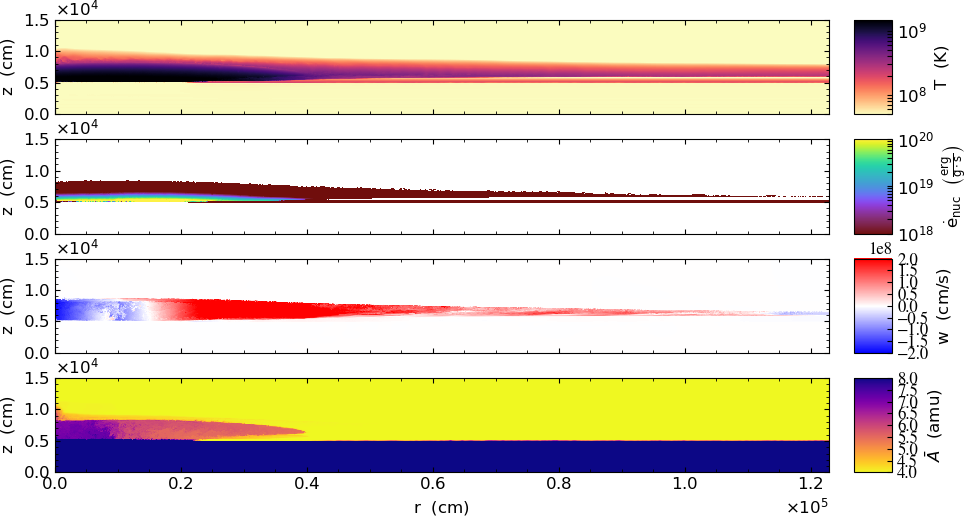
\includegraphics[width=0.75\linewidth]{xrb}
\caption{\label{fig:xrb} Helium flame spreading across the surface of
  a neutron star.  Shown are temperature (top), the velocity out of the
  simulation plane (middle), and nuclear energy generation rate
  (bottom).  }
\end{figure}

Figure~\ref{fig:xrb} shows a snapshot in time

\section{Estimates for Full Star Simulations}

A fully resolved calculation of burning over the entire neutron star
is out of reach, and will be for some time.

time estimate...

\MarginPar{Alice and Mike will work on this}


\section{Algorithmic Developments}

Algorithmic improvements are needed to push the scale of simulations
to the point where we can model XRBs at the full star scale with
resolved nuclear physics.  Here we discuss a few possibilities.

Machine architectures are evolving, with heterogeneous architectures
becoming more common.  Our recent development in \castro\ has focused
on moving the hydrodynamics to GPUs~\cite{astronum:2017}.  The XRB
problem is an ideal case for this, since hydrodynamics with constant
gravity (for plane-parallel domains) ports in a straightforward manner
to GPUs.  We can expect GPUs to perform 10--20$\times$ faster than
CPUs on modern supercomputer nodes.  This performance increase will
directly benefit XRB simulations.  GPU offloading of the reaction networks
will also allow us to explore larger networks and more detailed nuclear
physics.

If we continue to resolve the flame structure, then we need algroithms
that can do so less expensively.  We can be smarter about our grid
refinement strategy, putting the finest grids only at the very base of
the burning layer, where the flame is the thinnest.  Using
well-balanced schemes can help us retain HSE in the lower refined
regions, reducing the number of zones needed to maintain fidelity.  We
can also explore initialize newly created fine grids ahread of the burning
with an understanding of hydrostatic equilibrium to allow us to only refine
the peak burning as the flame moves across the star.

Another way we can meet the resolution requirements is to use a more
accurate hydrodynamic method.  In particular, we are developing fully
fourth-order (in space and time) coupling of hydrodynamics and
reactions using the method of spectral deferred corrections in
\castro, instead of the more commonly employed Strang splitting.  This
provides us with two benefits.  First, the improved coupling actually
reduces the stiffness of the reactions, requiring fewer righthand side
calls and therefore reducing the expense of the
reactions. \MarginPar{need some refs here} Second, by moving to fourth
order, we may also be able to reduce our resolution requirements
needed for converged flames, and since computational work scales like
$(\Delta x)^4$ in 3D, this can save a lot of computer time.

As an example of the improvements in coupling between hydro and \MarginPar{Don can add some comments about startup costs?}
reactions, Figure~\ref{fig:sdc} shows the mass fraction of helium
behind a detonation over the course of 3 timesteps.  The points
represent individual calls to the righthand side function of our
reaction network (a 13-isotope $\alpha$-chain), and the density of
points indicates how hard the integrator is working.  We use the same
tolerances for both the Strang-split method and the SDC method.  For
the SDC method, we are using a second-order accurate method.  We
predict a time-centered advection term, $\Adv{\Uc}^{n+1/2}_i$ using
standard unsplit Godunov methods, but explicitly include a reactive
source term in the tracing of the interface states.  We can then solve
the reactive system, using this advective term as a
piecewise-constant-in-time source
\begin{equation}
\frac{d{\Uc_i}}{dt} = -\Adv{\Uc}^{n+1/2}_i + {\bf R}(\Uc_i)
\end{equation}
This system can be integrated with standard ODE methods.  To achieve
second-order accuracy, we need to iterate, using the updated $\Uc$ to
create a reactive source included in the predictor for the advective
update, and then reintegrate the system.  The result of this iteration
is that the advection sees the effects of reactions over the timestep
and the reactions see the effects of advection.  For the zone tracked
in Figure~\ref{fig:sdc}, each SDC iteration called the righthand side
function of the network 5 times less than the Strang case.  
We are continuing to develop this new integration strategy, with full
fourth-order in space and time reacting hydrodynamics methods to
follow shortly.

\begin{figure}
\centering
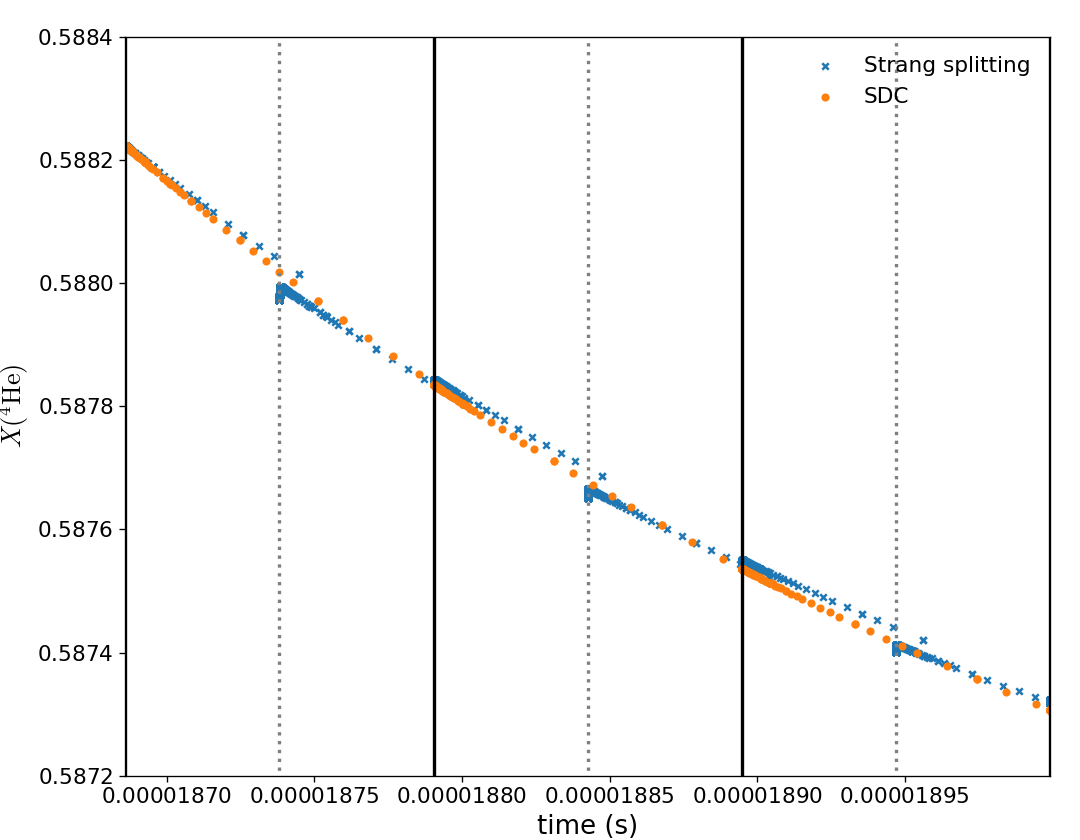
\includegraphics[width=0.75\linewidth]{sdc_plot}
\caption{\label{fig:sdc} Helium mass fraction as a function of time over three timesteps.}
\end{figure}


Other ways to make the simulation less expensive can include a subgrid model,
even something as simple as subzone burning.\MarginPar{need the paper ref fo rthis}

Finally, we can try hybrid model approaches where the fully
compressible simulation can act as a subgrid model.  \MarginPar{this ties into Ann's stuff, and also the stuff Alice was doing}


\section{Summary}

\ack The work at Stony Brook was supported by DOE/Office of Nuclear
Physics grant DE-FG02-87ER40317 and contract 7418390 with Lawrence
Berkeley National Laboratory as part of the Exascale Compute Project
ExaStar collaboration..  The work at LBNL was supported by the DOE
Office of Advanced Scientific Computing Research under Contract No,
DE-AC02-05CH11231. An award of computer time was provided by the
Innovative and Novel Computational Impact on Theory and Experiment
(INCITE) program.  This research used resources of the Oak Ridge
Leadership Computing Facility at the Oak Ridge National Laboratory,
which is supported by the Office of Science of the U.S. Department of
Energy under Contract No.\ DE-AC05-00OR22725.  This research used
resources of the National Energy Research Scientific Computing Center,
which is supported by the Office of Science of the U.S. Department of
Energy under Contract No.\ DE-AC02-05CH11231.  Visualizations were
done using yt~\cite{yt}.  This research has made use of NASA's
Astrophysics Data System Bibliographic Services.


\section*{References}

\bibliographystyle{iopart-num}
\bibliography{ws}


\end{document}
